\documentclass[11pt,letterpaper]{article}
\usepackage{samstyle}

\title{Ejercicios de programación}
        
\author{
	Profesores:\\[0.5cm]
	Sergio Andrés Monsalve Castañeda\\
	smonsal3@eafit.edu.co\\[1cm]
    John Jairo Silva Zuluaga \\
    jsilvazu@eafit.edu.co
}

\begin{document}
 
\pagestyle{fancyplain}
\fancyhf{}
\headheight=20pt %para cambiar el tamaño del encabezado
\renewcommand{\headrulewidth}{0pt} %espesor del encabezado

% \lhead %la "L" indica a la izquierda
% {
% }

\fancyfoot[c]{\thepage}

\maketitle

%\begin{minipage}{3cm}
% 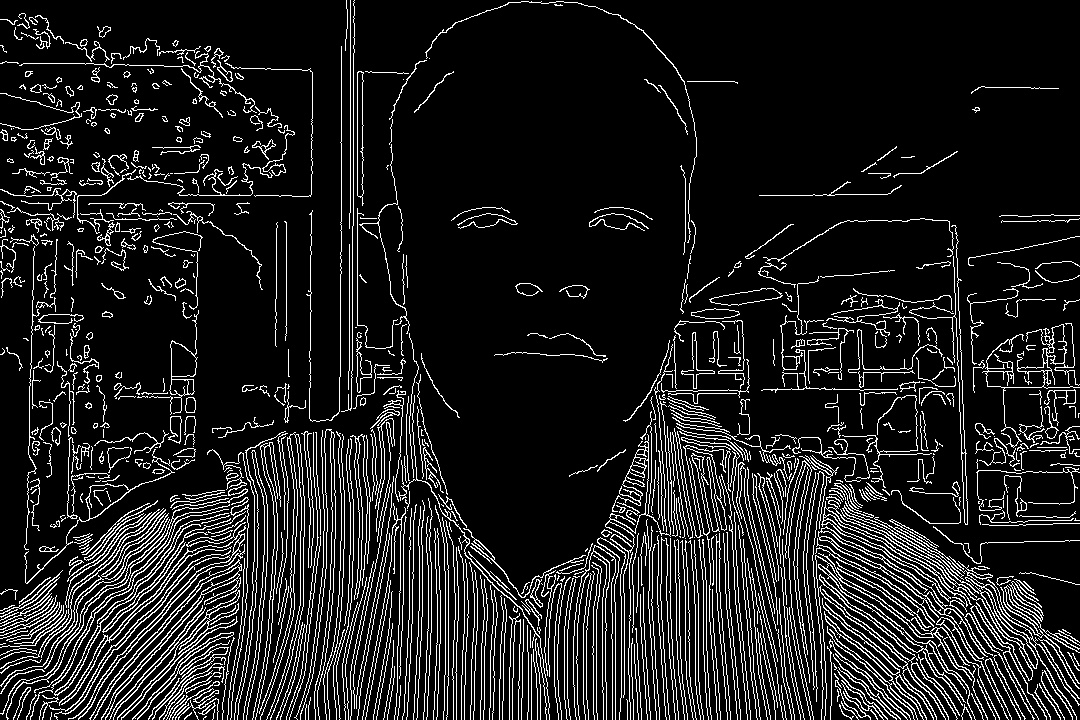
\includegraphics[width=15cm]{aux/SamCanny.jpg}
%\end{minipage}

\section{Problema 1: Ranking}

\subsection{Descripción}
Colombia hizo una apuesta amistosa con Venezuela sobre la participacion en los juegos Olimpicos. Cada país recibe medeallas de Oro, Plata y Bronce. Los paises son rankeados de dos maneras diferentes, o por la cantidad total de medallas (independiente de su tipo) o por el la cantidad de medallas que obtuvieron de oro, si estan enpatados en oro la cantidad de medallas de plata y si estan empatados en medallas de Plata, la cantidad de  Bronce.

Dada la catidad de medeallas de Oro / Plata / Bronce  para Colombia y Venezuela su objetivo es determinar si Colombia Gana en estos dos metodos. 

\subsubsection{Entrada}

La entrada esta compuesta por enteros consecutivos, los tres primeros corresponden a Colombia y los siguientes tres a venezuela, en el orden Oro, Plata, Bronce respectivamente.

\subsubsection{Salida}

Su programa de imprimir Cantidad, Tipo, Ambos o Ninguno, dependiendo de la modalidad en la que Colombia Gane de la siguiente manera.
Si Colombia tiene mas medallas en total que Venezuela, imprima Cantidad. Se gana por Tipo si Colombia tiene mas medallas de Oro que Venezuela, Si estan empatados entonces debe tener mas de Plata y si estan empatados debe tener mas de Bronce. 


\subsection{Ejemplo}

\begin{tabu} to \linewidth {|X[c]|X[c]|}
  \hline
  \rowfont{\bfseries\itshape\large} Entrada & Salida \\
  \hline
  \lstinputlisting{in2.in} & \lstinputlisting{ol.ot} \\
  \hline  
\end{tabu}


\begin{enumerate}
        \item A partir de 5 números, obtener su promedio y mostrar el entero mas cercano por encima. 
        Ejemplo: para 10, 8, 14, 2, 3 el promedio es 7.4, se mostraría el número 8.
        
        \item a partir de una lista de valores(vector o lista), hallar el promedio y la desviación estándar.
        
        \item Leer dos puntos en el espacio cartesiano, decir cual es la distancia entre ellos.
        
        \item Calcular la combinatoria de M y N, si $\dbinom{M}{N}$ = $\frac{M!}{N!(M-N)!}$
        
        \item Desarrolle una función en la cuál dados dos números (m y n), imprima un rectangulo de n x m '*' 
        
        \item Implemente una funcion que calcule Área y perímetro de un rectángulo (dos parámetros)
        
        \item Implemente una funcion que calcule Área y perímetro de un triángulo (3 parámetros)
        
        \item Implemente una funcion que calcule Área y perímetro de un círculo (se pasan 1 parámetro)
        
        \item Implemente una funcion que calcule Volumen y área de un cilindro( 2 parámetros)
        
        \item Dados 'n' números, imprimir, la suma del mayor y del menor
        
        \item Escribir un programa que diga si un número es capicúa (Un número capicúa es el que se puede leer igual al derecho y al revés)(Hacerlo sin transformar a cadena de caracteres)
        
        \item Pide por teclado un número entero positivo (debemos validarlo) y muestra  el número de cifras que tiene. Por ejemplo: si introducimos 1250, nos muestra que tiene 4 cifras.
        
        \item Dado un número mayor que 0 que representa cuantidad de segundos retornar cuantas horas, minutos y segundos hay, ejemplo: para el número 15723 imprimirá: 4 horas, 22 minutos y 3 segundos.
        
        \item Del anterior, hacer lo contrario, es decir, dados 3 valores(horas, minutos y segundos), escribir el número de segundos.
        
        \item Dados dos números: si los números son positivos, restarlos, si son negatívos, multiplicarlos, si son diferentes, dividirlos.
        
        \item Dados N números, imprimirlos en orden descendente
        
        \item Dados dos números enteros positivos N y D, se dice que D es un divisor de N si el residuo de dividir N entre D es 0. Se dice que un número N es perfecto si la suma de sus divisores (excluido el propio N) es N. Por ejemplo 28 es perfecto, pues sus divisores (excluido el 28) son: 1, 2, 4, 7 y 14 y su suma es 1+2+4+7+14=28. Hacer un programa que dado un número N nos diga si es o no perfecto.
        
        \item Un año es bisiesto si es múltiplo de 4, exceptuando los múltiplos de 100, que sólo son bisiestos cuando son múltiplos además de 400, por ejemplo el año 1900 no fue bisiesto, pero el año 2000 si lo será. Hacer un programa que dado un año A nos diga si es o no bisiesto.
        
        \item Hacer un programa que dados dos números(los catetos de un triángulo rectángulo), entregue el valor de la hipotenusa.
        
        \item A partir de 3 números naturales, decir si estos corresponden a un triángulo equilátero, isósceles o escaleno.
        
        \item Escribir los números que son múltiplos de 3 y de 7, del 1 al 1000

    \end{enumerate}
%\bibliographystyle{plainnat}
%\bibliography{refs}

\end{document}


